%! Author = Len Washington III
%! Date = 9/8/25

% Preamble
\documentclass[
	lecture={2},
	title={Birth of the Earth}
]{enve201notes}

% Packages

% Document
\begin{document}

\setcounter{chapter}{1}
%<*Lecture-2>
\chapter{Birth of the Earth}\label{ch:birth-of-the-earth}

\section{Scientific Cosmology}\label{sec:scientific-cosmology}
\begin{itemize}
	\item The systematic study of the overall structure and history of the Universe.
	\item The Universe contains two basic entities:
	\begin{description}
		\item[Matter] -- the substance that makes up objects
		\item[Energy] -- the inherent ability of a region of space and the matter \win\ it to do ``work''
	\end{description}
	\item In this lecture, we will learn
	\begin{itemize}
		\item Architecture of the overall Universe (including our Solar System)
		\item Formation of the Universe -- Big Bang Theory
		\item Production of Sun, the Earth, and other celestial objects
	\end{itemize}
\end{itemize}

\section{Structure of the Universe}\label{sec:structure-of-the-universe}
\subsection{Galaxies}\label{subsec:galaxies}
\begin{itemize}
	\item An immense group of \textbf{stars} held together by gravity.
	\item Our sun is one of over 300 billion \textbf{stars} in the Milky Way Galaxy.
\end{itemize}

\subsection{Star}\label{subsec:star}
\begin{itemize}
	\item An immense sphere of incandescent gas that emits intense energy.
	\item Stars, including our sun, are distant from each other, but all share similar structures.
\end{itemize}

\subsection{Solar System}\label{subsec:solar-system}
\begin{itemize}
	\item The Sun's gravitational pull holds many objects in orbit, forming the Solar System.
	\item Approximately 99.8\% of the Solar System's mass is contained \win\ the Sun; the remaining 0.2\% consists of a wide variety of objects.
	\item Solar System includes \emph{planets}, \emph{moons}, \emph{asteroids}, \emph{dwarf planets}, and \emph{comets}.
\end{itemize}

\subsection{Planets}\label{subsec:planets}
\begin{itemize}
	\item The astronomers' definition of a planet:
	\begin{enumerate}[label=\arabic*)]
		\item An object that orbits a star
		\item Roughly spherical
		\item Cleared its neighborhood of other objects (planet's gravity has pulled in all particles of matter in its orbit)
	\end{enumerate}
	\item Solar system includes eight planets:
	\begin{itemize}
		\item Mercury, Venus, Earth, Mars, Jupiter, Saturn, Uranus and Neptune
	\end{itemize}
	\item Until 2005, astronomers considered Pluto to be a planet.
	\begin{itemize}
		\item Why is Pluto's planet status revoked?
		\item Pluto has not cleared its orbit!
	\end{itemize}
\end{itemize}

\begin{figure}[H]
	\centering
	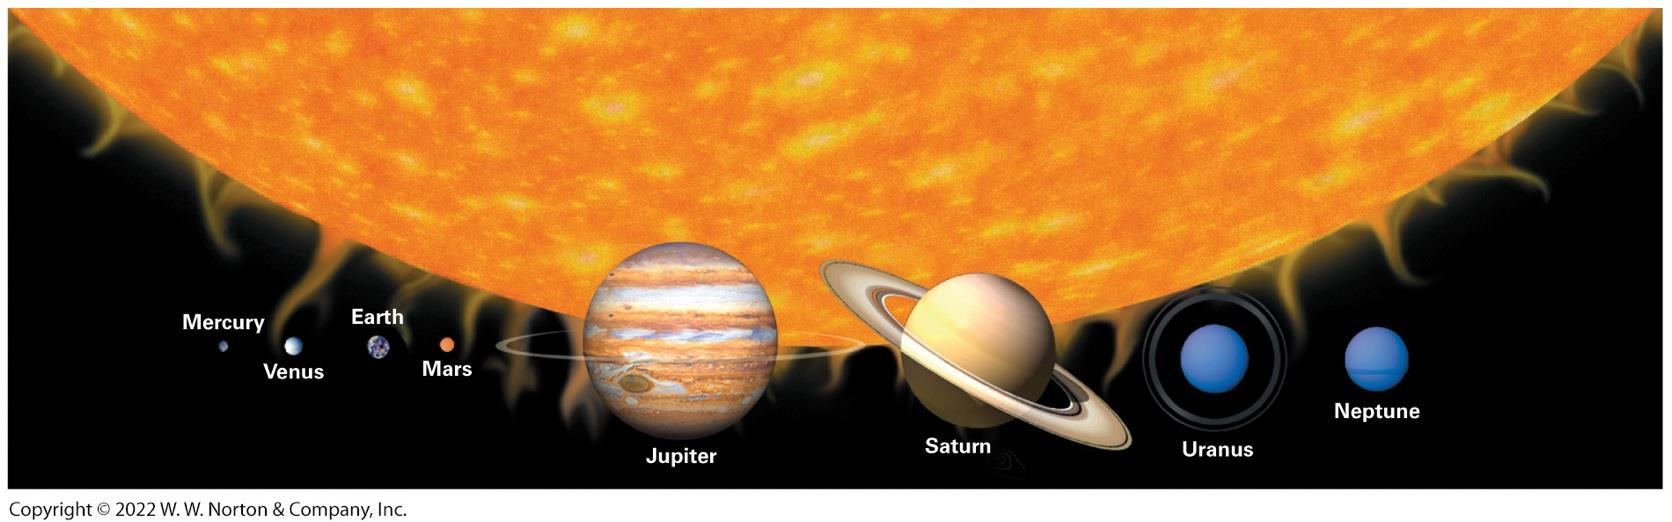
\includegraphics[width=\textwidth]{images/2_relative_sizes}
	\caption{Relative sizes of the planets.}
	\label{fig:relative-planet-sizes}
\end{figure}

\begin{figure}[H]
	\centering
	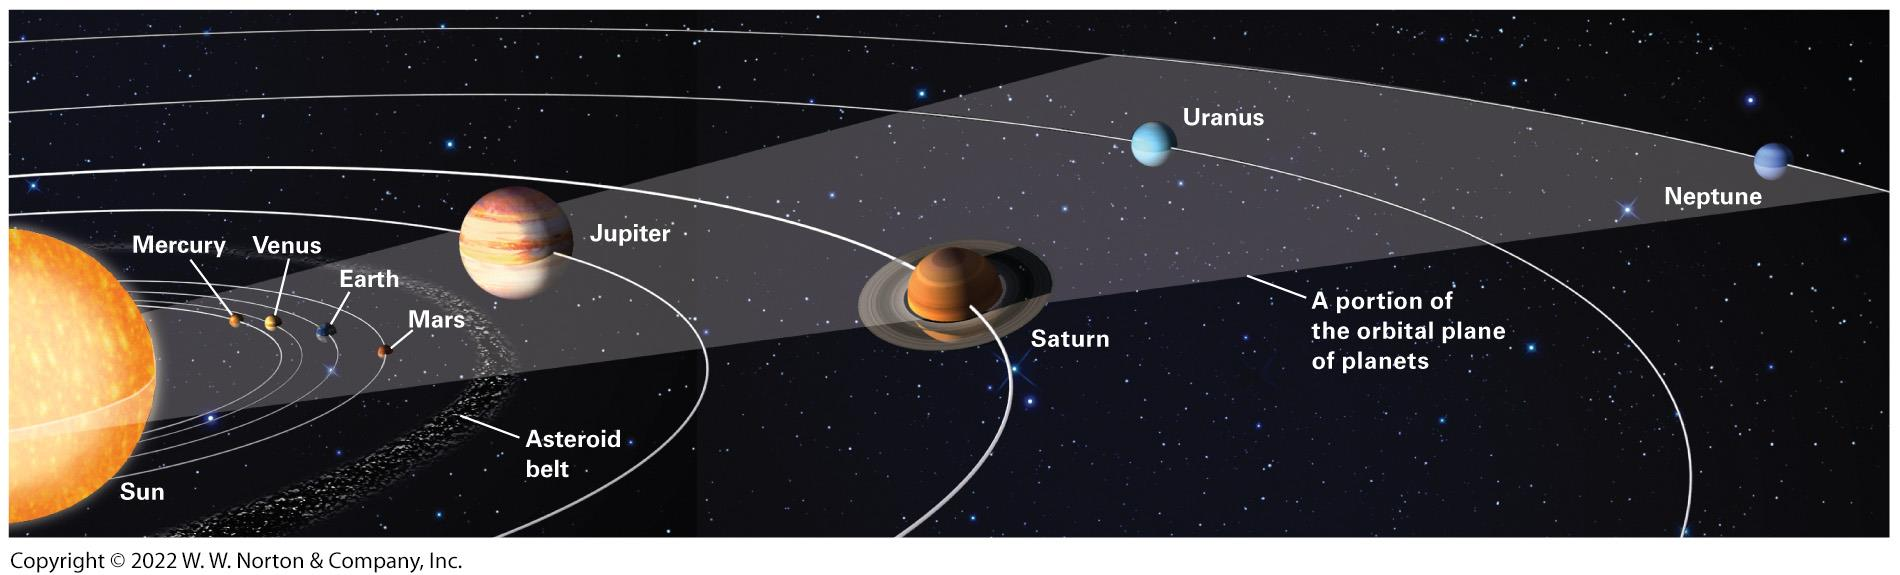
\includegraphics[width=\textwidth]{images/2_relative_positions}
	\caption{Relative positions of the planets.}
	\label{fig:relative-planet-positions}
\end{figure}

All planetary orbits lie roughly in the same plane.

\subsubsection{Terrestrial Planets (inner planets)}{subsubsec:terrestrial-planets}
\begin{itemize}
	\item Mercury, Venus, Earth, and Mars
	\item Closer to the Sun \& relatively small
	\item A shell of rock surrounding a ball of metal
\end{itemize}

\subsubsection{Giant Planets (outer planets)}{subsubsec:giant-planets}
\begin{itemize}
	\item Jupiter, Saturn, Uranus, and Neptune
	\item Most of the matter in Jupiter and Saturn consists of hydrogen and helium as a gas, liquid, or as a strange liquid-metal state -- referred to as \emph{gas giants}.
	\item Most of the matter in Neptune and Uranus consists of water, carbon dioxide, and methane that has been frozen into solid ice -- referred to as \emph{ice giants}.
\end{itemize}

\subsection{Moons}\label{subsec:moons}
\begin{itemize}
	\item A solid object that orbits a planet.
	\item All planets except Mercury and Venus have moons.
	\begin{itemize}
		\item Earth has the Moon.
		\item Mars has two.
		\item Jupiter has at least 63.
		\item Saturn has at least 62.
	\end{itemize}
	\item Moons vary greatly in size, composition, and surface characteristics.
\end{itemize}

\subsection{Other Objects}\label{subsec:other-objects}
\subsubsection{Asteroids}{subsubsec:asteroids}
\begin{itemize}
	\item Relatively small rocky or metallic objects that orbits the Sun.
	\item Most lie in the region between the orbits of Mars and Jupiter.
\end{itemize}

\subsubsection{Kuiper Belt and Oort Cloud Objects}{subsubsec:kuiper-belt-and-oort-cloud-objects}
\begin{itemize}
	\item A trillion icy bodies that form a donut-like ring \textbf{outside Neptune's orbit} make up the Kuiper Belt.
	\item More distant ones form the spherical-shaped Oort Cloud.
\end{itemize}

\subsubsection{Dwarf Planets}{subsubsec:dwarf-planets}
\begin{itemize}
	\item Asteroids and Kuiper Belt objects \w\ a diameter greater than $\sim900$ km.
	\item Maybe up to 200 dwarf planets present, only five have yet been identified.
	\item Pluto and Eris are the largest known dwarf planets.
\end{itemize}

\subsubsection{Comets}{subsubsec:comets}
\begin{itemize}
	\item Kuiper Belt and Oort Cloud objects that follow elliptical orbits that bring them into the inner Solar System.
\end{itemize}

\section{Formation of the Universe -- The Big Bang}\label{sec:formation-of-the-universe-the-big-bang}
\begin{itemize}
	\item According to the Big Bang Theory, all matter and energy in the Universe was initially concentrated in an infinitesimally small point.
	\item This point suddenly exploded, making the beginning of the Universe.
	\item The initial expansion, known as the inflation epoch, occurred extremely rapidly and lasted less than a second.
	\item Following this brief period, the Universe continued to expand (at a slower rate).
\end{itemize}

\begin{figure}[H]
	\centering
	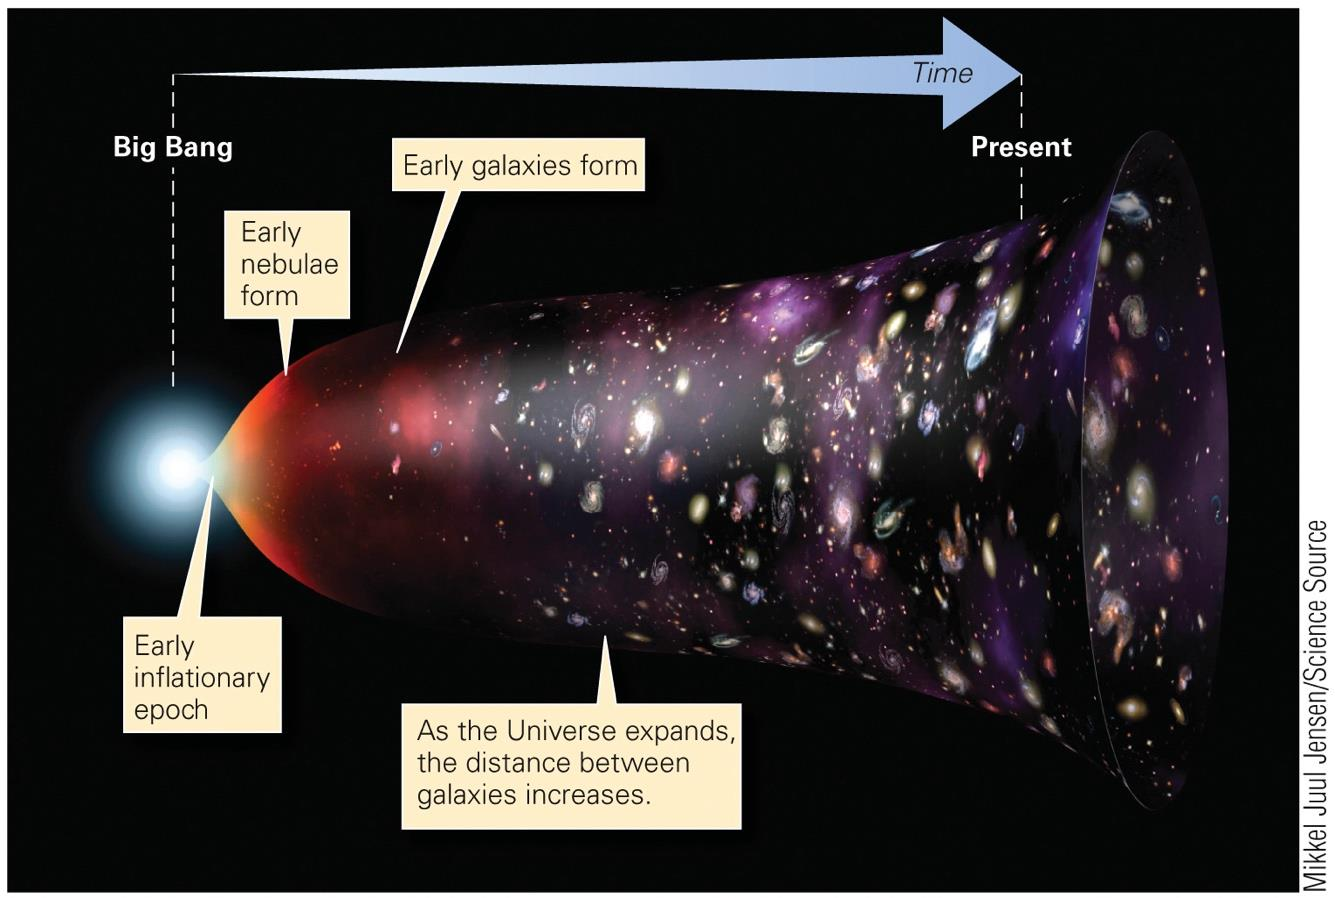
\includegraphics[width=\textwidth]{images/2_big_bang}
	\caption{The concepts of the expanding Universe and the Big Bang.}
	\label{fig:big-bang-concepts}
\end{figure}

\section{Birth of the First Stars}\label{sec:birth-of-the-first-stars}
\begin{itemize}
	\item By the time the Universe reached its 200 millionth year, it was filled \w\ immense, slowly swirling dark nebulae--giant clouds of dust and gas--separated by vast, empty voids.
\end{itemize}

\begin{figure}[H]
	\centering
	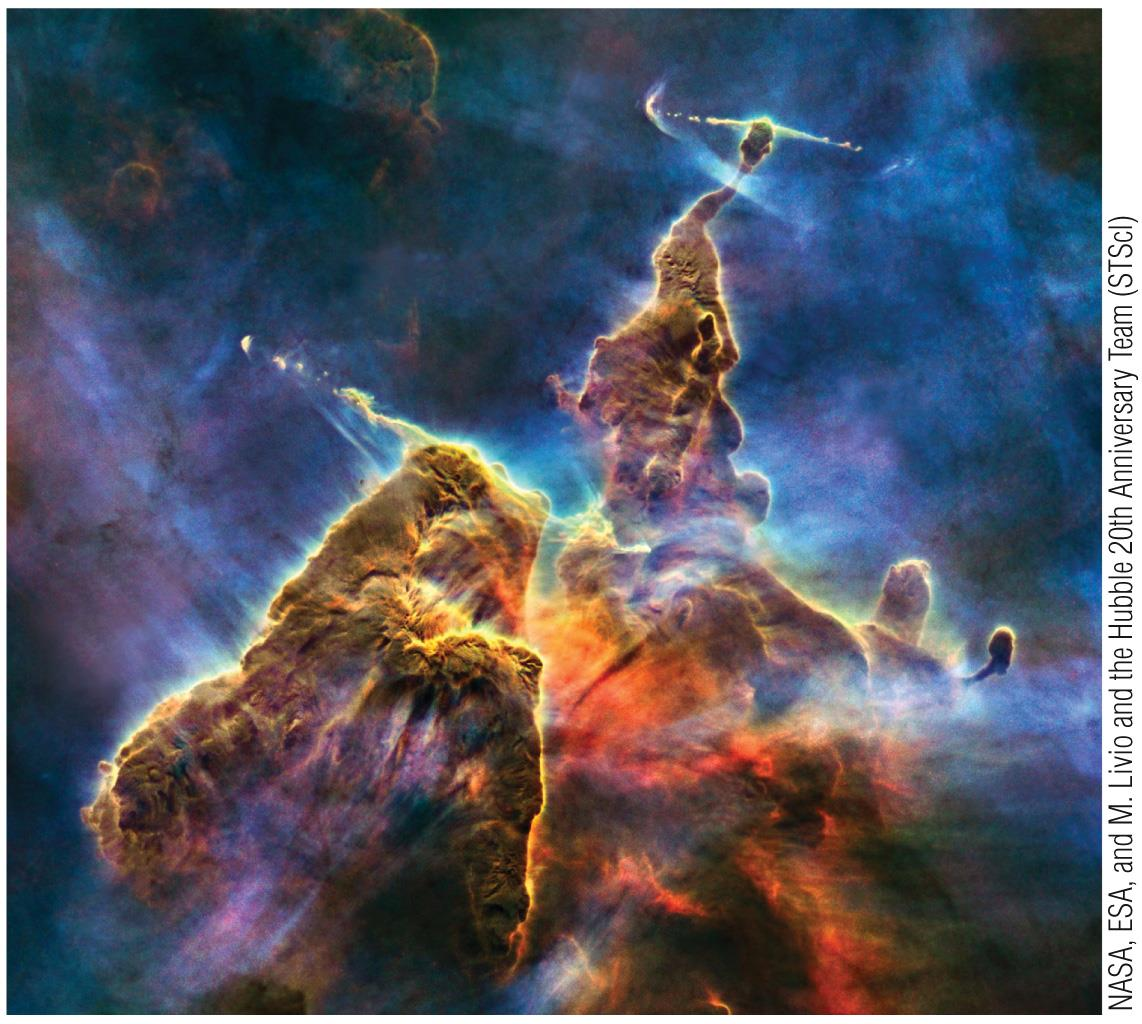
\includegraphics[width=\textwidth]{images/2_starless_nebulae}
	\caption{A representation of a starless nebula in the early Universe (modified from a Hubble Space Telescope photograph)}
	\label{fig:starless-nebulae}
\end{figure}

\subsection{Formation Process}\label{subsec:formation-process}
\begin{itemize}
	\item \W\ the gravitational pull, a nebula began to draw in surrounding ice and gas, increasing its mass and density.
	\item As it grew, the cloud's slow swirling motion transformed into a rotation around a central axis, forming a disk-like shape.
	\item As gravity continued to pull material inward, the inner region of the disk collapsed into a dense, hot core.
	\item Eventually, the core became hot enough to emit light--this glowing core marked the birth of a \emph{protostar}.
\end{itemize}

\subsection{From Protostar to Star}\label{subsec:from-protostar-to-star}
\begin{itemize}
	\item As the protostar accumulated more mass, its core grew even denser and hotter.
	\item Under these extreme conditions, hydrogen nuclei began to move rapidly and fuse into helium in a process known as nuclear fusion.
	\item Once fusion began, the protostar ignited, and the first true star was born.
	\item Around 800 million years after the Big Bang, stars lit up the Universe.
	\item This process repeated over and over, giving rise to the first generation of stars, marking a new era in cosmic evolution.
\end{itemize}

\section{Supernova}\label{sec:supernova}
\begin{itemize}
	\item The larger the star, the hotter it burns, and the faster it runs out of fuel and dies.
	The explosion of a giant star produces a supernova!
\end{itemize}

\subsection{Crab Nebula}\label{subsec:crab-nebula}
\begin{itemize}
	\item One of the largest ever taken by NASA's Hubble Space Telescope.
	\item A six-light-year-wide expanding remnant of a star's supernova explosion.
	\item Japanese and Chinese astronomers recorded this violent event in 1054 CE.
\end{itemize}

\section{Formation of the Solar System -- The Nebular Theory}\label{sec:the-nebular-theory}
\begin{itemize}
	\item How the planets and other objects in our Solar System originated?
	\item \definition{The nebular theory (or condensation theory)}{the Sun and all other objects in the Solar System formed from material that had been swirling about in a nebula.}
	\item Tiny particles of ice and dust condensed \win\ a nebula.
	\item Gradually, more atoms and molecules stuck to these particles, forming larger clumps.
	\item Once these clumps grow big enough, their gravity pulled them together, growing into even larger bodies.
	\item As gravity pulled the swirling gas and dust inward, the nebula flattened into a spinning disk with a dense, central region.
	\item This central ``bulb'' became the \emph{Sun}, while the rest of the disk became the \emph{protoplanetary disk}.
	\item \Win\ this disk, dust and rocky debris collided and stuck together to form \emph{planetesimals}.
	\item These planetesimals, acting like vacuum cleaner, attracted more material and gew into \emph{protoplanets}--early versions of the planets we see today.
\end{itemize}

\section{Differentiation of the Earth's Interior}\label{sec:differentiation-of-the-earth's-interior}
\begin{itemize}
	\item Early on, the composition of the Earth (planetesimals) was fairly uniform.
	\item When temperatures got hot enough, iron began to melt.
	\item Then, the iron accumulated at the center of the planet to create the core.
\end{itemize}

\section{Formation of the Moon}\label{sec:formation-of-the-moon}
\begin{itemize}
	\item Soon after the Earth formed, a protoplanet collided \w\ Earth, blasting debris around it, and the Moon formed from the ring of debris.
\end{itemize}

\section{Formation of Earth's Ocean and Atmosphere}\label{sec:formation-of-earth's-ocean-and-atmosphere}
\begin{itemize}
	\item Unlike the other terrestrial planets, Earth is unique for having liquid water oceans and an atmosphere rich in nitrogen (\ce{N2}) and oxygen (\ce{O2}).
	However, this wasn't always the case.
\end{itemize}

\subsection{Earth's Early Atmosphere}\label{subsec:earth's-early-atmosphere}
\begin{itemize}
	\item When Earth first formed, its atmosphere likely consisted mostly of lightweight gases--hydrogen (\ce{H2}) and helium (\ce{He})--similar to the Sun.
	\begin{itemize}
		\item Where did hydrogen and helium go?
		\item Where did the ocean and atmosphere come from?
	\end{itemize}
\end{itemize}
%
\begin{itemize}
	\item As the planet warmed, the initial light gases--hydrogen (\ce{H2}) and helium (\ce{He}) -- escaped Earth's gravitational pull.
	\item These were replaced by gases released through volcanic eruptions, known as \emph{volatile materials}.
	This outgassing from Earth's interior led to the formation of a new atmosphere, primarily composed of water vapor, carbon dioxide (\ce{CO2}), ammonia (\ce{NH3}), and methane (\ce{CH4}).
	\item When the Earth cooled enough for water vapor to condense, rain \emph{began to fall} and the \emph{oceans gradually accumulated}.
	\item \emph{\ce{CO2} dissolved into the oceans} and \emph{precipitated as solid compounds}, reducing its concentration in the atmosphere.
	\item Later, \emph{photosynthetic organisms} emerged, gradually increasing oxygen (\ce{O2}) in the atmosphere and changing Earth's environment dramatically.
\end{itemize}
%</Lecture-2>
\end{document}